\chapter{Probabilités}

\minitoc

\section{Dénombrabilité}

\subsection{Vocabulaire}

\begin{defi}
On dit qu'un ensemble \(E\) est dénombrable quand il existe une bijection de \(\N\) dans \(E\).
\end{defi}

Dans ce cas, cela signifie qu'on peut numéroter les éléments de \(E\) par les entiers naturels et donc qu'on peut écrire \(E\) en extension sous une forme \(E=\accol{x_n\tq n\in\N}\) sans jamais répéter deux fois le même élément : on dit qu'on a énuméré les éléments de \(E\).

Un ensemble fini est de la forme \(\accol{x_0,\dots,x_n}\) : on peut aussi l'écrire sous la forme \(\accol{x_n\tq n\in\N}\) en répétant une infinité de fois au moins un élément. C'est pourquoi on voit souvent dans les raisonnements apparaître la locution \guillemets{ensemble fini ou dénombrable} ou \guillemets{ensemble au plus dénombrable}.

Évidemment, tout ensemble en bijection avec un ensemble dénombrable est aussi dénombrable, car une composée de bijections est une bijection.

\subsection{Exemples}

\begin{prop}
\begin{itemize}
    \item \(\N\), \(\Ns\), plus généralement \(\intervie{n_0}{\pinf}\inter\N\) (pour tout \(n_0\in\N\)), et encore plus généralement toute partie infinie de \(\N\) sont dénombrables. \\
    \item \(\Z\) est dénombrable. \\
    \item \(\quantifs{\Tpt p\in\Ns}\N^p\text{ est dénombrable}\). \\
    \item \(\Q\) est dénombrable. \\
    \item Si \(\paren{u_i}_{i\in I}\) est une famille sommable de complexes, alors le support de la famille \(\accol{i\in I\tq u_i\not=0}\) est dénombrable.
\end{itemize}
\end{prop}

\begin{dem}
\begin{itemize}
    \item Si \(A\) est une partie infinie de \(\N\), on construit une énumération de \(A\) par \guillemets{l'algorithme} suivant : \[u_0=\min A\qquad\text{et}\qquad\quantifs{\forall n\in\N}u_{n+1}=\min\paren{A\excluant\accol{u_0,\dots,u_n}}.\]
    \item On peut représenter \(\Z\) de la manière suivante, avec en bas les éléments de \(\Z\) et en haut les étiquettes : \begin{center}
    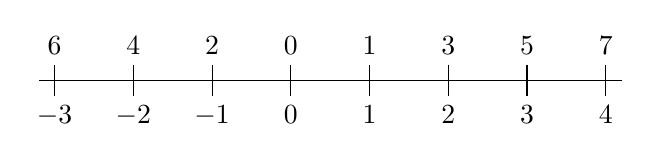
\begin{tikzpicture}
        \draw (-3.2,0) -- (4.2,0);
        \draw (-3,0.2) node[above] {\(6\)} -- (-3,-0.2) node[below] {\(-3\)};
        \draw (-2,0.2) node[above] {\(4\)} -- (-2,-0.2) node[below] {\(-2\)};
        \draw (-1,0.2) node[above] {\(2\)} -- (-1,-0.2) node[below] {\(-1\)};
        \draw (0,0.2) node[above] {\(0\)} -- (0,-0.2) node[below] {\(0\)};
        \draw (1,0.2) node[above] {\(1\)} -- (1,-0.2) node[below] {\(1\)};
        \draw (2,0.2) node[above] {\(3\)} -- (2,-0.2) node[below] {\(2\)};
        \draw (3,0.2) node[above] {\(5\)} -- (3,-0.2) node[below] {\(3\)};
        \draw (4,0.2) node[above] {\(7\)} -- (4,-0.2) node[below] {\(4\)};
    \end{tikzpicture}
    \end{center}
    On en déduit que \(\fonction{\phi}{\N}{\Z}{n}{\paren{-1}^{n+1}\floor{\dfrac{n+1}{2}}}\) est une bijection de \(\N\) dans \(\Z\) dont la bijection réciproque est \(\fonctionlambda{\Z}{\N}{p}{\begin{dcases}-2p &\text{si }p\leq0 \\ 2p-1 &\text{sinon}\end{dcases}}\) \\
    \item On peut représenter \(\N^2\) de la manière suivante : \begin{center}
        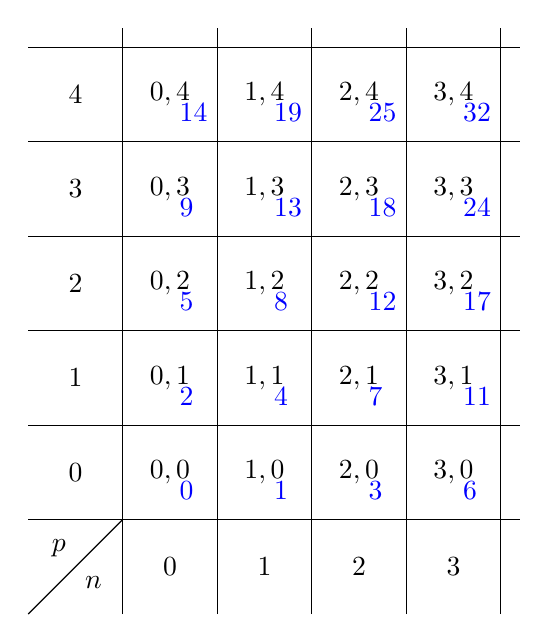
\begin{tikzpicture}[scale=1.2]
            \draw (0,0) -- (1,1);

            \draw (0,1) -- (5.2,1);
            \draw (0,2) -- (5.2,2);
            \draw (0,3) -- (5.2,3);
            \draw (0,4) -- (5.2,4);
            \draw (0,5) -- (5.2,5);
            \draw (0,6) -- (5.2,6);

            \draw (1,0) -- (1,6.2);
            \draw (2,0) -- (2,6.2);
            \draw (3,0) -- (3,6.2);
            \draw (4,0) -- (4,6.2);
            \draw (5,0) -- (5,6.2);

            \node[below right] at (0.5,0.5) {\(n\)};
            \node[above left] at (0.5,0.5) {\(p\)};

            \node at (1.5,0.5) {\(0\)};
            \node at (2.5,0.5) {\(1\)};
            \node at (3.5,0.5) {\(2\)};
            \node at (4.5,0.5) {\(3\)};

            \node at (0.5,1.5) {\(0\)};
            \node at (0.5,2.5) {\(1\)};
            \node at (0.5,3.5) {\(2\)};
            \node at (0.5,4.5) {\(3\)};
            \node at (0.5,5.5) {\(4\)};

            \node at (1.5,1.5) {\(\paren{0,0}\)};
            \node at (1.5,2.5) {\(\paren{0,1}\)};
            \node at (1.5,3.5) {\(\paren{0,2}\)};
            \node at (1.5,4.5) {\(\paren{0,3}\)};
            \node at (1.5,5.5) {\(\paren{0,4}\)};
            \node at (2.5,1.5) {\(\paren{1,0}\)};
            \node at (2.5,2.5) {\(\paren{1,1}\)};
            \node at (2.5,3.5) {\(\paren{1,2}\)};
            \node at (2.5,4.5) {\(\paren{1,3}\)};
            \node at (2.5,5.5) {\(\paren{1,4}\)};
            \node at (3.5,1.5) {\(\paren{2,0}\)};
            \node at (3.5,2.5) {\(\paren{2,1}\)};
            \node at (3.5,3.5) {\(\paren{2,2}\)};
            \node at (3.5,4.5) {\(\paren{2,3}\)};
            \node at (3.5,5.5) {\(\paren{2,4}\)};
            \node at (4.5,1.5) {\(\paren{3,0}\)};
            \node at (4.5,2.5) {\(\paren{3,1}\)};
            \node at (4.5,3.5) {\(\paren{3,2}\)};
            \node at (4.5,4.5) {\(\paren{3,3}\)};
            \node at (4.5,5.5) {\(\paren{3,4}\)};
            
            \node[below right,blue] at (1.5,1.5) {\(0\)};
            \node[below right,blue] at (1.5,2.5) {\(2\)};
            \node[below right,blue] at (1.5,3.5) {\(5\)};
            \node[below right,blue] at (1.5,4.5) {\(9\)};
            \node[below right,blue] at (1.5,5.5) {\(14\)};
            \node[below right,blue] at (2.5,1.5) {\(1\)};
            \node[below right,blue] at (2.5,2.5) {\(4\)};
            \node[below right,blue] at (2.5,3.5) {\(8\)};
            \node[below right,blue] at (2.5,4.5) {\(13\)};
            \node[below right,blue] at (2.5,5.5) {\(19\)};
            \node[below right,blue] at (3.5,1.5) {\(3\)};
            \node[below right,blue] at (3.5,2.5) {\(7\)};
            \node[below right,blue] at (3.5,3.5) {\(12\)};
            \node[below right,blue] at (3.5,4.5) {\(18\)};
            \node[below right,blue] at (3.5,5.5) {\(25\)};
            \node[below right,blue] at (4.5,1.5) {\(6\)};
            \node[below right,blue] at (4.5,2.5) {\(11\)};
            \node[below right,blue] at (4.5,3.5) {\(17\)};
            \node[below right,blue] at (4.5,4.5) {\(24\)};
            \node[below right,blue] at (4.5,5.5) {\(32\)};
        \end{tikzpicture}
    \end{center}
    On en déduit que \(\fonction{\phi}{\N^2}{\N}{\paren{n,p}}{\dfrac{\paren{n+p}\paren{n+p+1}}{2}+p}\) est une bijection de \(\N^2\) dans \(\N\) dont la réciproque est définie comme suit. \\\\ Pour \(N\in\N\), on pose \(k=\max\accol{i\in\N\tq\dfrac{i\paren{i+1}}{2}\leq N}\) puis \(p=N-k\) et \(n=k-p\), et enfin \(N\mapsto\paren{n,p}\). \\\\ Autre bijection possible : on a unicité de la décomposition \(\quantifs{\forall n\geq1}n=2^a\paren{2b+1}\) où \(\paren{a,b}\in\N^2\) \ie \(\fonction{\psi}{\Ns}{\N^2}{n}{\paren{a,b}}\) est une bijection et donc \(\isomorphismelambda{\N}{\N^2}{n}{\psi\paren{n+1}}\). \\
    \item Si on considère \(\phi_2\) une bijection de \(\N^2\) dans \(\N\), \[\begin{array}[t]{ccccccc}\N^3 & \xrightarrow{\;\sim\;} & \N\times\N^2 & \xrightarrow{\;\sim\;} & \N\times\N & \xrightarrow{\;\sim\;} & \N \\ \paren{a,b,c} & \mapsto & \paren{a,\paren{b,c}} & \mapsto & \paren{a,\phi_2\paren{b,c}} & \mapsto & \phi_2\paren{a,\phi_2\paren{b,c}}\end{array}\] est une bijection de \(\N^3\) dans \(\N\). \\\\ Par récurrence, si \(\phi_p\) est une bijection de \(\N^p\) dans \(\N\), alors \[\isomorphisme{\phi_{p+1}}{\N^{p+1}}{\N}{\paren{a_1,\dots,a_{p+1}}}{\phi_2\paren{a_1,\phi_p\paren{a_2,\dots,a_{p+1}}}}\] est une bijection de \(\N^{p+1}\) dans \(\N\). \\
    \item Tout \(x\in\Qs\) s'écrit de façon unique sous forme irréductible \(x=\dfrac{p}{q}\) où \(\paren{p,q}\in\Z\times\Ns\) tel que \(p\et q=1\), donc \[\fonctionlambda{\Z\times\Ns}{\Qs}{\paren{p,q}}{\dfrac{p}{q}}\] est bijective. \\\\ Donc \(\Q\simeq\Qs\simeq\Z\times\Ns\simeq\N^2\simeq\N\) (où \(\simeq\) est la relation d'équipotence). \\
    \item Soit \(\paren{u_i}_{i\in I}\) une famille sommable de complexes. \\\\ On pose \(S=\Supp\paren{u_i}=\accol{i\in I\tq u_i\not=0}\). \\ \begin{itemize}
        \item Si \(S\) est fini, alors \(S\) est au plus dénombrable. \\
        \item Si \(S\) est infini, pour \(k\in\Ns\), on pose \(S_k=\accol{i\in I\tq\abs{u_i}>\dfrac{1}{k}}\) et on a \(S=\bigunion_{k\in\Ns}S_k\). \\\\ Montrons que \(\quantifs{\tpt k\in\Ns}S_k\) est fini. \\\\ Soient \(k\in\Ns\) et \(\paren{i_1,\dots,i_p}\in S_k^p\) distincts. \\\\ Pour \(j\in\interventierii{1}{p}\), on a \(\abs{u_{i_j}}\geq\dfrac{1}{k}\) donc \[\sum_{j=1}^p\abs{u_{i_j}}\geq\dfrac{p}{k}.\] Or \(\paren{u_i}_{i\in I}\) est sommable donc il existe \(M>0\) tel que \(\quantifs{\tpt J\in\Pf{I}}\sum_{j\in J}\abs{u_j}\leq M\). \\\\ On a donc \(\dfrac{p}{k}\leq\sum_{j=1}^p\abs{u_{i_j}}\leq M\), et donc \(p\leq Mk\). \\\\ Si \(S_k\) est infini, on peut choisir \(\floor{Mk}+1\) éléments distincts de \(S_k\) donc \(\floor{Mk}+1\leq Mk\) d'après ce qui précède : contradiction. \\\\ Donc \(S_k\) est fini. \\\\ On peut donc numéroter les éléments de \(S_k\) via \(\phi_k:S_k\to\interventierii{0}{N_k}\). \\\\ Pour \(i\in S\), on pose \(m_i=\min\accol{k\in\Ns\tq i\in S_k}\) et à \(i\) on peut associer le couple \(\paren{m_i,\phi_{m_i}\paren{i}}\). \\\\ On construit ainsi une injection de \(S\) dans \(\N^2\), donc par composition avec une bijection de \(\N^2\) dans \(\N\), une injection de \(S\) dans \(\N\), \ie \(S\) est en bijection avec une partie infinie de \(\N\). \\\\ Donc \(S\) est en bijection avec \(\N\).
    \end{itemize}
\end{itemize}
\end{dem}

En revanche, il existe des ensembles infinis non-dénombrables, comme \(\R\) ou tout intervalle de longueur non-nulle. Un ensemble non-dénombrable est trop gros pour qu'on puisse ordonner ses éléments et les numéroter.

\begin{dem}[\(\R\) n'est pas dénombrable]
Tout réel \(x\) peut s'écrire de manière unique sous la forme \[x=p+\sum_{k=0}^{\pinf}\dfrac{c_k}{10^k}\] où \(p=\floor{x}\in\Z\) et \(\paren{c_k}\in\interventierii{0}{9}^\N\) n'est pas stationnaire en \(9\). On peut écrire \(x=p,c_1c_2\dots c_n\dots\)

Par l'absurde, si \(\intervie{0}{1}\) est dénombrable, on peut numéroter les réels de \(\intervie{0}{1}\) : \(x_0,x_1,\dots,x_n,\dots\)

On a \[\begin{aligned}
x_0&=0,c_{0,1}c_{0,2}c_{0,3}\dots \\
x_1&=0,c_{1,1}c_{1,2}c_{1,3}\dots \\
&\vdots \\
x_n&=0,c_{n,1}c_{n,2}c_{n,3}\dots c_{n,n+1} \\
&\vdots
\end{aligned}\]

On choisit \(d_1\in\interventierii{0}{8}\) tel que \(d_1\not=c_{0,1}\), \(d_2\in\interventierii{0}{8}\) tel que \(d_2\not=c_{1,2}\), etc., \(d_n\in\interventierii{0}{8}\) tel que \(d_n\not=c_{n,n+1}\) puis on pose \[y=0,d_1d_2\dots d_n\dots=\sum_{k=1}^{\pinf}\dfrac{d_k}{10^k}.\]

Donc \(y\in\intervie{0}{1}\).

Or, par construction, \(y\not\in\accol{x_0,\dots,x_n,\dots}=\intervie{0}{1}\) : contradiction.
\end{dem}

\subsection{Quelques propriétés}

\begin{prop}
Toute partie infinie d'un ensemble dénombrable est dénombrable.

Si \(E\) est dénombrable, alors pour toute injection de \(F\) dans \(E\), \(F\) est au plus dénombrable.
\end{prop}

Pourvu qu'on ne considère pas trop d'ensembles, les réunions d'ensembles dénombrables le sont aussi.

\begin{prop}
Si \(E_1,\dots,E_n\) sont (au plus) dénombrables, alors \(E_1\union\dots\union E_n\) l'est aussi.

Si \(\paren{E_i}_{i\in I}\) est une famille (au plus) dénombrable d'ensembles (au plus) dénombrables, alors \(\bigunion_{i\in I}E_i\) l'est aussi.
\end{prop}

En revanche, pour les produits cartésiens, il faut se contenter d'un nombre fini d'ensembles.

\begin{prop}
Si \(E_1,\dots,E_n\) sont dénombrables, alors \(E_1\times\dots\times E_n\) est dénombrable.
\end{prop}

En revanche, un produit cartésien quelconque d'ensembles dénombrables ne l'est pas en général : par exemple, \(\accol{0,1}^\N\) n'est pas dénombrable.

\section{Espace probabilisé}

\subsection{Univers d'une expérience aléatoire}

Une expérience aléatoire est une expérience dont on connaît les résultats possibles (les issues possibles) mais dont on ne peut pas connaître à l'avance le résultat. On modélise l'expérience par la donnée de l'ensemble \(\Omega\) des issues possibles.

\begin{defi}
L'ensemble des issues possibles est appelé univers des possibles (ou univers). Il est souvent noté \(\Omega\).
\end{defi}

\begin{ex}
\begin{itemize}
    \item On jette un dé non-truqué : les issues possibles sont les six entiers \(1,\dots,6\) ; l'univers est donc \(\Omega=\accol{1,\dots,6}\). \\
    \item On jette \(n\) fois un dé : les issues possibles sont les suites de \(n\) entiers de l'ensemble \(\accol{1,\dots,6}\) ; donc \(\Omega=\interventierii{1}{6}^n\). \\
    \item On lance une pièce une infinité de fois : les issues possibles sont les suites infinies de \(0\) ou \(1\) ; donc \(\Omega=\accol{0,1}^\N\).
\end{itemize}
\end{ex}

\subsection{Tribu d'événements}

De manière informelle, un événement est une partie de l'univers \(\Omega\). Mais cette définition est trop vague. Si on autorise toutes les parties de l'univers à être des événements, alors quand l'ensemble \(\Omega\) est infini non-dénombrable, les seules probabilités sur \(\Omega\) sont des probabilités discrètes (théorème d'Ulam), ce qui exclut tout un tas de probabilités intéressantes. Donc on doit en général restreindre la notion d'événement à certaines parties de \(\Omega\) : certaines parties n'ont donc pas le droit d'être nommées \guillemets{événement}.

\begin{defi}
Soit \(\Omega\) un univers.

On appelle tribu sur \(\Omega\) une partie \(\fami{T}\) de \(\P{\Omega}\) telle que :

\begin{itemize}
    \item \(\Omega\in\fami{T}\) \\
    \item \(\quantifs{\tpt A\in\fami{T}}\conj{A}\in\fami{T}\) \\
    \item pour toute suite \(\quantifs{\paren{A_n}\in\fami{T}^\N}\bigunion_{n\in\N}A_n\in\fami{T}\).
\end{itemize}
\end{defi}

Modéliser une expérience aléatoire, c'est choisir l'univers et une tribu : les éléments de la tribu sont appelés les événements. On dit qu'un événement est réalisé quand l'issue de l'expérience aléatoire appartient à cet événement. Le couple \(\groupe{\Omega}[\fami{T}]\) est appelé espace probabilisable.

\begin{ex}
\begin{itemize}
    \item L'ensemble \(\accol{\ensvide,\Omega}\) est une tribu, c'est la plus petite tribu envisageable. Elle est inutilisable en pratique car elle ne comporte pas assez d'événements pour décrire des situations issues de la vie réelle. \\
    \item L'ensemble \(\P{\Omega}\) est une tribu : quand l'univers \(\Omega\) est fini ou dénombrable, c'est la tribu utilisée systématiquement, mais quand \(\Omega\) est infini non-dénombrable, c'est une tribu trop grosse pour pouvoir y définir une probabilité vraiment utile. \\
    \item En école d'ingénieur, vous entendrez parler de la tribu des boréliens : c'est celle qui est couramment utilisée quand \(\Omega=\R\).
\end{itemize}
\end{ex}

\begin{prop}
Soient \(\Omega\) un ensemble et \(\fami{T}\) une tribu sur \(\Omega\).

Alors on a :

\begin{itemize}
    \item \(\ensvide\in\fami{T}\) \\
    \item pour toute suite \(\quantifs{\paren{A_n}\in\fami{T}^\N}\biginter_{n\in\N}A_n\in\fami{T}\) \\
    \item pour toute famille finie \(\paren{A_1,\dots,A_n}\) d'événements, \(\bigunion_{k=0}^nA_k\) et \(\biginter_{k=0}^nA_k\) sont des événements.
\end{itemize}
\end{prop}

\begin{dem}
Soit \(\paren{A_n}\in\fami{T}^\N\).

On a \(\biginter_{n\in\N}A_n\in\fami{T}\) car \[\biginter_{n\in\N}A_n=\conj{\bigunion_{n\in\N}\conj{A_n}}.\]
\end{dem}

\begin{defi}
\(\Omega\) est appelé l'événement certain, \(\ensvide\) est appelé l'événement impossible.

Deux événements \(A\) et \(B\) sont dits incompatibles quand ils sont disjoints, \ie \(A\inter B=\ensvide\).
\end{defi}

\subsection{Probabilité}

\begin{defi}
Soient \(\Omega\) un univers et \(\fami{T}\) une tribu sur \(\Omega\).

On appelle probabilité sur \(\groupe{\Omega}[\fami{T}]\) toute application \(\prem:\fami{T}\to\intervii{0}{1}\) telle que :

\begin{itemize}
    \item \(\proba{\Omega}=1\) \\
    \item pour toute suite \(\paren{A_n}\in\fami{T}^\N\) d'événements deux à deux incompatibles, la série de terme général \(\proba{A_n}\) est convergente et \(\proba{\bigsqcup_{n\in\N}A_n}=\sum_{n=0}^{\pinf}\proba{A_n}\).
\end{itemize}

Le triplet \(\anneau{\Omega}[\fami{T}][\prem]\) est appelé espace probabilisé.
\end{defi}

En pratique, sauf dans certains cas où \(\Omega\) est fini ou dénombrable, nous postulerons toujours l'existence d'un espace probabilisé qui modélise la situation, car c'est hors de notre portée de construire concrètement un tel espace. Dès que les expériences aléatoires peuvent avoir une infinité non-dénombrable de résultats possibles, il est souvent difficile de reprendre les idées développées en première année et définir, par exemple, des probabilités à partir d'événements élémentaires \(\accol{\omega}\) (définir \(\Omega\) est en général à notre portée, mais construire la tribu et la probabilité est inaccessible à nos moyens). Nous admettrons donc toujours l'existence d'un espace probabilisé représentant notre expérience.

Dans moult cas, nous définirons les événements à partir d'événements \guillemets{primitifs} : par exemple, dans le cas d'une suite de lancer de pièce, l'univers est simple : \(\accol{0,1}^\N\), mais il n'est pas dénombrable ; les événements primitifs sont les événements \(P_i\), où \(i\in\N\) et \[P_i=\accol{\omega=\paren{\omega_n}\in\accol{0,1}^\N\tq\omega_i=1}\] modélise l'événement au sens concret \guillemets{obtenir pile au \(i\)-ème lancer}.

\begin{exo}
On lancer une pièce une infinité de fois.

Exprimez par une phrase ce que représentent les événements suivants : \[A_n=\biginter_{i=0}^nP_i\qquad B_n=\bigunion_{i=0}^n\paren{P_i\inter\biginter_{\substack{0\leq j\leq n \\ j\not=i}}\overline{P_j}}\qquad C=\bigunion_{i\in\N}\biginter_{j\geq i}P_j.\]

Réciproquement, définissez à l'aide des \(P_i\) les événements suivants :

\begin{itemize}
    \item on obtient pile un nombre fini de fois \\
    \item on obtient pile une infinité de fois.
\end{itemize}
\end{exo}

\begin{corr}
\begin{itemize}
    \item \(\omega\in A_n\ssi\) \guillemets{on obtient pile lors des \(n+1\) premiers lancers}. \\
    \item \[\begin{aligned}
        \omega\in B_n&\ssi\quantifs{\exists i\in\interventierii{0}{n}}\omega\in P_i\inter\biginter_{\substack{0\leq j\leq n \\ i\not=j}}\conj{P_j} \\
        &\ssi\quantifs{\exists i\in\interventierii{0}{n}}\croch{\omega\in P_i\quad\text{et}\quad\quantifs{\forall j\in\interventierii{0}{n}\excluant\accol{i}}\omega\in\conj{P_j}} \\
        &\ssi\text{ \guillemets{parmi les \(n+1\) premiers lancers, un seul donne pile}}.
    \end{aligned}\]
    \item \(\omega\in C\ssi\) \guillemets{à partir d'un certain rang, on obtient uniquement pile}. \\
    \item \guillemets{On obtient pile un nombre fini de fois} \(\ssi\omega\in\bigunion_{i\in\N}\biginter_{j\geq i}\conj{P_j}=D\). \\
    \item \guillemets{On obtient pile une infinité de fois} \(\ssi\omega\in\conj{D}=\biginter_{i\in\N}\bigunion_{j\geq i}P_j\).
\end{itemize}
\end{corr}

\subsection{Propriétés}

On retrouve les propriétés vues en première année.

\begin{prop}\thlabel{prop13.6}
Soit \(\anneau{\Omega}[\fami{T}][\prem]\) un espace probabilisé.

Alors \(\prem\) vérifie les propriétés suivantes :

\begin{itemize}
    \item \(\quantifs{\tpt A\in\fami{T}}\proba{\overline{A}}=1-\proba{A}\) ; en particulier \(\proba{\ensvide}=0\) \\
    \item \(\quantifs{\tpt\paren{A,B}\in\fami{T}^2}A\subset B\imp\proba{A}\leq\proba{B}\) \\
    \item \(\quantifs{\tpt\paren{A,B}\in\fami{T}^2}\proba{A\union B}=\proba{A}+\proba{B}-\proba{A\inter B}\).
\end{itemize}
\end{prop}

Mais on en a d'autres, liées à la notion de suite dénombrable.

\subsubsection{Continuité}

\begin{prop}[Continuité croissante]
Si \(\paren{A_n}\) est une suite croissante d'événements, \cad \(\quantifs{\tpt n\in\N}A_n\subset A_{n+1}\), alors \[\proba{\bigunion_{n\in\N}A_n}=\lim_{n\to\pinf}\proba{A_n}.\]
\end{prop}

\begin{dem}
Soit \(\paren{A_n}\) une suite croissante d'événements.

On pose \(B_0=A_0\) et \(\quantifs{\tpt n\in\N}B_n=A_n\excluant A_{n-1}\).

On vérifie d'abord que \(\bigunion_{i\in\N}B_i=\bigunion_{i\in\N}A_i\) : \begin{itemize}
    \item \(\quantifs{\Tpt n\in\N}B_n\subset A_n\) donc \(\bigunion_{n\in\N}B_n\subset\bigunion_{n\in\N}A_n\). \\
    \item Soit \(\omega\in\bigunion_{i\in\N}A_i\). \\\\ Alors \(\accol{k\in\N\tq\omega\in A_k}\) est une partie non-vide de \(\N\) et possède donc un minimum \(i\in\N\). \\\\ Donc, si \(i\geq1\), alors \(i-1\) n'appartient pas à cet ensemble. \\\\ Ainsi, ou bien \(i=0\) et \(\omega\in B_0\), ou bien \(i\not=0\) et \(\omega\in A_i\) et \(\omega\not\in A_{i-1}\) donc \(\omega\in B_i\). \\\\ Donc \(\omega\in\bigunion_{n\in\N}B_n\) et donc \(\bigunion_{n\in\N}A_n\subset\bigunion_{n\in\N}B_n\). \\
\end{itemize}

De plus, les événements \(B_i\) sont deux à deux incompatibles \ie \[\quantifs{\forall\paren{i,j}\in\N^2}i\not=j\imp B_i\inter B_j=\ensvide.\]

En effet, soit \(\paren{i,j}\in\N^2\) tel que \(i>j\).

Si \(\omega\in B_i\inter B_j\), alors \(\omega\in B_j\subset A_j\subset\dots\subset A_{i-1}\).

Or \(\omega\in B_i=A_i\excluant A_{i-1}\) donc \(\omega\not\in A_{i-1}\) : contradiction.

Donc \(B_i\inter B_j=\ensvide\).

D'après la deuxième propriété de \(\prem\), \(\proba{\bigsqcup_{i\in\N}B_i}=\sum_{i\in\N}\proba{B_i}\) donc \[\proba{\bigunion_{i\in\N}A_i}=\sum_{i\in\N}\proba{B_i}=\sum_{i=0}^{\pinf}\proba{B_i}.\]

Or \(B_i=A_i\excluant A_{i-1}\) et \(A_{i-1}\subset A_i\) donc \[A_i=A_{i-1}\sqcup B_i.\]

Donc \(\proba{B_0}=\proba{A_0}\) et pour \(i\geq1\) on a \[\begin{aligned}
\proba{A_i}&=\proba{A_{i-1}}+\proba{B_i} \\
\proba{A_i}-\proba{A_{i-1}}&=\proba{B_i}.
\end{aligned}\]

Donc \[\begin{aligned}
\proba{\bigunion_{i\in\N}A_i}&=\lim_{N\to\pinf}\sum_{i=0}^N\proba{B_i} \\
&=\lim_{N\to\pinf}\croch{\sum_{i=1}^N\paren{\proba{A_i}-\proba{A_{i-1}}}+\proba{A_0}} \\
&=\lim_{N\to\pinf}\paren{\proba{A_0}+\proba{A_N}-\proba{A_0}} \\
&=\lim_{N\to\pinf}\proba{A_N}.
\end{aligned}\]
\end{dem}

\begin{prop}[Continuité décroissante]
Si \(\paren{A_n}\) est une suite décroissante d'événements, \cad \(\quantifs{\tpt n\in\N}A_{n+1}\subset A_n\), alors \[\proba{\biginter_{n\in\N}A_n}=\lim_{n\to\pinf}\proba{A_n}.\]
\end{prop}

\begin{dem}
Soit \(\paren{A_n}\) une suite décroissante d'événements.

Alors \(\paren{\conj{A_n}}\) est croissante.

Donc \(\proba{\bigunion_{n\in\N}\conj{A_n}}=\lim_{n\to\pinf}\proba{\conj{A_n}}\).

Donc \(1-\proba{\bigunion_{n\in\N}\conj{A_n}}=\lim_{n\to\pinf}\paren{1-\proba{\conj{A_n}}}\).

Donc \(\proba{\conj{\bigunion_{n\in\N}\conj{A_n}}}=\lim_{n\to\pinf}\proba{A_n}\).

Donc \(\proba{\biginter_{n\in\N}A_n}=\lim_{n\to\pinf}\proba{A_n}\).
\end{dem}

\begin{prop}\thlabel{prop13.9}
Soit \(\paren{A_n}\) une suite quelconque d'événements. On a \[\proba{\bigunion_{n=0}^{\pinf}A_n}=\lim_{N\to\pinf}\proba{\bigunion_{n=0}^NA_n}\qquad\text{et}\qquad\proba{\biginter_{n=0}^{\pinf}A_n}=\lim_{N\to\pinf}\proba{\biginter_{n=0}^NA_n}.\]
\end{prop}

\begin{dem}
Pour \(n\in\N\), on pose \(A_n\prim=\bigunion_{k=0}^nA_k\).

La suite \(\paren{A_n\prim}\) est croissante et \(\bigunion_{n\in\N}A_n\prim=\bigunion_{n\in\N}A_n\).

D'après la proposition de continuité croissante, on a donc \[\proba{\bigunion_{n\in\N}A_n}=\proba{\bigunion_{n\in\N}A_n\prim}=\lim_{n\to\pinf}\proba{A_n\prim}.\]

Idem pour l'intersection avec la continuité décroissante.
\end{dem}

\begin{exo}
On considère l'univers des suites infinies de lancers indépendants d'une pièce équilibrée : \(\Omega=\accol{0,1}^\N\).

Montrez que les événements élémentaires \(\accol{\omega}\) sont de probabilité nulle.

Déduisez-en que l'univers n'est pas dénombrable.

Quelle est la probabilité d'obtenir un nombre fini de face ?
\end{exo}

\begin{corr}
\begin{itemize}
    \item On considère par exemple l'événement \guillemets{on n'obtient que des piles} \(=A\). \\\\ \(A=\biginter_{i\in\N}P_i=\accol{\paren{1,1,1,\dots,1,\dots}}\) est un événement élémentaire. \\\\ D'après la \thref{prop13.9}, on a \(\proba{A}=\lim_{n\to\pinf}\proba{\biginter_{i=0}^nP_i}\). \\\\ Or les événements \(P_i\) sont indépendants et \(\proba{P_i}=\dfrac{1}{2}\) donc \[\proba{\biginter_{i=0}^nP_i}=\prod_{i=0}^n\proba{P_i}=\paren{\dfrac{1}{2}}^{n+1}.\] Donc \(\proba{A}=\lim_{n\to\pinf}\dfrac{1}{2^{n+1}}=0\). \\
    \item Soient \(\omega\in\Omega\) et \(A=\accol{\omega}=\accol{\paren{\omega_0,\omega_1,\dots,\omega_n,\dots}}=\biginter_{i\in\N}B_i\) où \(B_i=\begin{dcases}
        P_i &\text{si }\omega_i=1 \\
        \conj{P_i} &\text{si }\omega_i=0
    \end{dcases}\) \\\\ D'après la \thref{prop13.9}, on a \[\proba{A}=\lim_{n\to\pinf}\proba{\biginter_{i=0}^nB_i}=\lim_{n\to\pinf}\dfrac{1}{2^{n+1}}=0.\]
    \item Supposons \(\Omega=\accol{0,1}^\N\) dénombrable. \\\\ On a \(\Omega=\bigsqcup_{\omega\in\Omega}\accol{\omega}\). \\\\ L'union étant dénombrable, on a \[1=\proba{\Omega}=\sum_{\omega\in\Omega}\proba{\accol{\omega}}=0\] contradiction. \\\\ Donc \(\accol{0,1}^\N\) n'est pas dénombrable. \\
    \item Soit \(B\) l'événement \guillemets{on obtient un nombre fini de face}. On a \[B=\bigunion_{i\in\N}\underbrace{\biginter_{j\geq i}P_j}_{Q_i}.\] \(Q_i\) est l'événement \guillemets{on obtient que des pile à partir du rang \(i\)}. \\\\ Si \(\omega\in Q_i\), \(\quantifs{\forall j\geq i}\omega_j=1\) donc \(\quantifs{\forall j\geq i+1}\omega_j=1\), donc \(\omega\in Q_{i+1}\) \ie \(Q_i\subset Q_{i+1}\). \\\\ Donc \(\paren{Q_i}\) est croissante et on a \(\proba{B}=\lim_{i\to\pinf}\proba{Q_i}\). \\\\ Or \(Q_i=\biginter_{j\geq i}P_j\) donc \[\begin{aligned}
        \proba{Q_i}&=\lim_{N\to\pinf}\proba{\biginter_{j=i}^NP_j} \\
        &=\lim_{N\to\pinf}\paren{\dfrac{1}{2}}^{N-i+1} \\
        &=0.
    \end{aligned}\] Donc \(\proba{B}=0\).
\end{itemize}
\end{corr}

\subsubsection{Sous-additivité}

\begin{prop}[Sous-additivité]\thlabel{prop13.10}
Si \(\paren{A_n}\) est une suite d'événements, alors \[\proba{\bigunion_{n\in\N}A_n}\leq\sum_{n=0}^{\pinf}\proba{A_n}.\]
\end{prop}

\begin{dem}
D'après la \thref{prop13.6}, on a \[\quantifs{\forall\paren{A,B}\in\fami{T}^2}\proba{A\union B}=\proba{A}+\proba{B}-\proba{A\inter B}\leq\proba{A}+\proba{B}.\]

Puis, par récurrence, on a \[\quantifs{\forall n\in\Ns;\forall\paren{A_1,\dots,A_n}\in\fami{T}^n}\proba{\bigunion_{i=1}^nA_i}\leq\sum_{i=1}^n\proba{A_i}.\]

Donc \[\quantifs{\forall\paren{A_n}\in\fami{T}^\N;\forall k\in\N}\proba{\bigunion_{i=0}^kA_i}\leq\sum_{i=0}^k\proba{A_i}\leq\sum_{i=0}^{\pinf}\proba{A_i}.\]

Or, d'après la \thref{prop13.9}, on a \(\proba{\bigunion_{i\in\N}A_i}=\lim_{k\to\pinf}\proba{\bigunion_{i=0}^kA_i}\), donc par passage à la limite, on a \[\proba{\bigunion_{i\in\N}A_i}\leq\sum_{i=0}^{\pinf}\proba{A_i}.\]
\end{dem}

Dans ce résultat, le symbole \(\sum_{n=0}^{\pinf}\proba{A_n}\) signifie \(\lim_{N\to\pinf}\sum_{n=0}^N\proba{A_n}\) : c'est un réel si la série \(\sum\proba{A_n}\) est convergente, et \(\pinf\) sinon (puisque la série est à termes positifs).

\subsubsection{Événements négligeables ou presque sûrs}

\begin{defi}
Un événement est dit négligeable quand sa probabilité est nulle.

Un événement est dit presque sûr quand sa probabilité est \(1\).
\end{defi}

\begin{prop}
Toute réunion ou intersection au plus dénombrable d'événements négligeables est négligeable.

Toute réunion ou intersection au plus dénombrable d'événements presque sûrs est presque sûre.
\end{prop}

\begin{dem}
Application directe de la \thref{prop13.10}.
\end{dem}

\subsection{Probabilité discrète}

\begin{defi}
Soit \(\Omega\) un univers.

On appelle distribution de probabilité discrète sur \(\Omega\) toute famille de réels positifs indexée par \(\Omega\), sommable et de somme totale \(1\).

Si \(\Omega\) est un ensemble fini, on retrouve la définition de l'an dernier.
\end{defi}

\begin{prop}
Si \(\paren{p_\omega}_{\omega\in\Omega}\) est une distribution de probabilité discrète sur \(\Omega\), alors son support \(\accol{\omega\in\Omega\tq p_\omega>0}\) est au plus dénombrable.
\end{prop}

À toute distribution de probabilité discrète sur \(\Omega\), on peut associer une probabilité sur l'espace probabilisable \(\groupe{\Omega}[\P{\Omega}]\).

\begin{prop}
Si \(\paren{p_\omega}_{\omega\in\Omega}\) est une distribution de probabilité discrète sur \(\Omega\), alors il existe une unique probabilité \(\prem\) sur la tribu \(\P{\Omega}\) telle que \(\quantifs{\tpt\omega\in\Omega}\proba{\accol{\omega}}=p_\omega\).
\end{prop}

\begin{dem}
Soit \(\paren{p_\omega}_{\omega\in\Omega}\) une distribution de probabilité discrète.

Pour \(A\in\P{\Omega}\), on pose \(\proba{A}=\sum_{\omega\in A}p_\omega\) (au sens des familles sommables).

On a \(A\subset\Omega\) donc \(0\leq\proba{A}\leq\proba{\Omega}=\sum_{\omega\in\Omega}p_\omega=1\).

Donc \(\prem\) est une application de \(\P{\Omega}\) dans \(\intervii{0}{1}\) qui vérifie \(\proba{\Omega}=1\).

Soit \(\paren{A_n}_{n\in\N}\) une famille dénombrable de \(\P{\Omega}\) telle que \(\quantifs{\tpt\paren{m,n}\in\N^2}m\not=n\imp A_m\inter A_n=\ensvide\).

On veut montrer \(\proba{\bigunion_{n\in\N}A_n}=\sum_{n\in\N}\proba{A_n}\).

D'après le théorème de sommation par paquets, on a \[\begin{WithArrows}
\sum_{n\in\N}\proba{A_n}&=\sum_{n\in\N}\sum_{\omega\in A_n}p_\omega \Arrow{\(\paren{A_n}\) partition de \(\bigunion_{n\in\N}A_n\)} \\
&=\sum_{\omega\in\bigunion_{n\in\N}A_n}p_\omega \\
&=\proba{\bigunion_{n\in\N}A_n}.
\end{WithArrows}\]

\(\prem\) est donc une probabilité sur \(\P{\Omega}\) telle que \(\quantifs{\tpt\omega\in\Omega}\proba{\accol{\omega}}=p_\omega\).

Ceci prouve donc l'existence de \(\prem\).

Pour montrer l'unicité, soit \(Q\) une probabilité qui vérifie les conditions de l'énoncé.

On pose \(S\) le support \(Q\) : \(S=\accol{\omega\in\Omega\tq p_\omega>0}\).

Soit \(A\in\P{\Omega}\).

On a \(A=\paren{A\inter S}\sqcup\paren{A\inter\conj{S}}\) donc \[\begin{WithArrows}
Q\paren{A}&=Q\paren{A\inter S}+Q\paren{A\inter\conj{S}} \\
&=Q\paren{\bigsqcup_{\omega\in A\inter S}\accol{\omega}}+Q\paren{A\inter\conj{S}} \Arrow{\(A\inter S\) dénombrable} \\
&=\sum_{\omega\in A\inter S}Q\paren{\accol{\omega}}+Q\paren{A\inter\conj{S}} \\
&=\sum_{\omega\in A\inter S}p_\omega+Q\paren{A\inter\conj{S}}.
\end{WithArrows}\]

En particulier, si \(A=\Omega\), on a \[Q\paren{\Omega}=1=\sum_{\omega\in S}p_\omega+Q\paren{\conj{S}}.\]

Or, d'après le théorème de sommation par paquets, on a \[\sum_{\omega\in\Omega}p_\omega=1=\sum_{\omega\in S}p_\omega+\underbrace{\sum_{\omega\in\conj{S}}\underbrace{p_\omega}_{=0}}_{=0}.\]

Donc \(Q\paren{\conj{S}}=0\).

Donc \(0\leq Q\paren{A\inter\conj{S}}\leq Q\paren{\conj{S}}=0\) et donc \(Q\paren{A\inter\conj{S}}=0\).

Donc \(Q\paren{A}=\sum_{\omega\in A\inter S}p_\omega\).

Ceci est aussi valable pour la probabilité \(\prem\) donc \(\proba{A}=Q\paren{A}\).

Donc \(\prem=Q\).
\end{dem}

Quand l'univers est infini non-dénombrable, le résultat précédent donne toutes les probabilités discrètes sur \(\groupe{\Omega}[\P{\Omega}]\). Mais si on choisit des tribus plus petites (ce qui est très relatif : en général, ce sont des ensembles énormes, dont la puissance dépasse celle du continu !), alors on peut créer d'autres types de probabilités (comme les probabilités dites continues).

Quand l'univers \(\Omega\) est fini ou dénombrable, alors toutes les probabilités sont discrètes : on choisit toujours la tribu \(\P{\Omega}\), ce qui est toujours sous-entendu.

\begin{prop}
Soit \(\Omega=\accol{\omega_1,\dots,\omega_n}\) un ensemble fini.

Alors pour tout \(n\)-uplet \(\paren{p_1,\dots,p_n}\in\intervii{0}{1}^n\) tel que \(\sum_{i=1}^np_i=1\), il existe une unique probabilité \(\prem\) sur \(\Omega\) telle que \(\quantifs{\tpt i\in\interventierii{1}{n}}\proba{\accol{\omega_i}}=p_i\).
\end{prop}

\begin{prop}\thlabel{prop13.15}
Soit \(\Omega=\accol{\omega_1,\dots,\omega_n,\dots}\) un ensemble dénombrable.

Alors pour toute suite \(\paren{p_n}\in\intervii{0}{1}^\N\) telle que la série \(\sum_{n\geq1}p_n\) converge et \(\sum_{n=1}^{\pinf}p_n=1\), il existe une unique probabilité \(\prem\) sur \(\Omega\) telle que \(\quantifs{\tpt i\in\Ns}\proba{\accol{\omega_i}}=p_i\).
\end{prop}

\begin{exo}
Déterminez l'unique constante \(\lambda\) telle qu'on puisse définir une probabilité sur \(\N\) en posant \[\quantifs{\tpt n\in\N}\proba{\accol{n}}=\dfrac{\lambda}{n!}.\]
\end{exo}

\begin{corr}~\\
La famille \(\paren{\dfrac{\lambda}{n!}}_{n\in\N}\) est une distribution de probabilité discrète sur \(\N\) si et seulement si \[\begin{dcases}
\sum_{n\in\N}\dfrac{\lambda}{n!}=1 \\
\quantifs{\forall n\in\N}\dfrac{\lambda}{n!}\geq0
\end{dcases}\]

Or on a \(\sum_{n\in\N}\dfrac{\lambda}{n!}=\lambda\sum_{n=0}^{\pinf}\dfrac{1}{n!}=\lambda\e{}\) donc la seule solution est \(\lambda=\dfrac{1}{\e{}}\).
\end{corr}

Dans toute la suite, on suppose donné un espace probabilisé \(\anneau{\Omega}[\fami{T}][\prem]\).

\section{Probabilités conditionnelles}

\subsection{Généralités}

\begin{defi}
Soit \(A\in\fami{T}\) un événement non-négligeable.

Pour \(B\in\fami{T}\), on pose \(\probacond{B}{A}=\dfrac{\proba{A\inter B}}{\proba{A}}\), appelé probabilité sachant \(A\) de \(B\).
\end{defi}

On voit aussi la notation \(\proba{B\tq A}\), mais attention, cette notation est trompeuse, elle peut laisser penser qu'il existe un événement qui s'appellerait \guillemets{\(B\) sachant \(A\)}, ce qui n'a aucun sens.

L'idée derrière la notion de probabilité conditionnelle est que lorsqu'on dispose d'une information partielle sur le résultat de l'expérience, notre perception des probabilités s'en trouve modifiée.

\begin{theo}
Sous les mêmes hypothèses, \(\prem_A\) est une probabilité sur \(\groupe{\Omega}[\fami{T}]\), appelée probabilité conditionnelle relative à \(A\).
\end{theo}

\begin{dem}~\\
On a \(\probacond{\Omega}{A}=\dfrac{\proba{A\inter\Omega}}{\proba{A}}=\dfrac{\proba{A}}{\proba{A}}=1\).

Pour toute famille \(\paren{B_n}_{n\in\N}\) d'événements deux à deux incompatibles, on a \[\begin{aligned}
\probacond{\bigsqcup_{n\in\N}B_n}{A}&=\dfrac{1}{\proba{A}}\proba{A\inter\bigsqcup_{n\in\N}B_n} \\
&=\dfrac{1}{\proba{A}}\proba{\bigsqcup_{n\in\N}\paren{A\inter B_n}} \\
&=\dfrac{1}{\proba{A}}\sum_{n\in\N}\proba{A\inter B_n} \\
&=\sum_{n\in\N}\probacond{B_n}{A}.
\end{aligned}\]

Donc \(\prem_A\) est une probabilité sur \(\groupe{\Omega}[\fami{T}]\).
\end{dem}

En général, on connaît plutôt \(\proba{A}\) et \(\probacond{B}{A}\), ce qui permet de calculer \(\proba{A\inter B}\) : \[\proba{A\inter B}=\proba{A}\probacond{B}{A}.\]

On peut généraliser.

\begin{theo}[Formule des probabilités composées]
Soit \(\paren{A_1,\dots,A_n}\) une famille d'événements tels que \(\proba{A_1\inter\dots\inter A_{n-1}}\not=0\).

Alors \(\proba{A_1\inter\dots\inter A_{n-1}\inter A_n}=\proba{A_1}\probacond{A_2}{A_1}\probacond{A_3}{A_1\inter A_2}\dots\probacond{A_n}{A_1\inter\dots\inter A_{n-1}}\).
\end{theo}

En général, on utilise ce résultat lorsque des événements (au sens naturel) se succèdent et que la connaissance de chaque événement permet de déterminer l'état du système.

\begin{exo}
On dispose d'une urne contenant une boule blanche et \(n\) boules noires (avec \(n\geq1\)).

On effectue une suite de tirages jusqu'à obtenir la boule blanche en respectant le protocole suivant : si on tire une boule noire, on la remplace par deux boules noires.

Calculez la probabilité d'obtenir la boule blanche à l'issue du \(k\)-ème tirage et la probabilité de ne jamais tirer la boule blanche.
\end{exo}

\begin{corr}
Pour \(k\in\Ns\), on note \(A_k\) l'événement \guillemets{on tire une boule noire au \(k\)-ème tirage} et \(B_k\) l'événement \guillemets{on tire la boule blanche au \(k\)-ème tirage}.

On a \[B_k=\biginter_{i=1}^{k-1}A_i\inter\conj{A_k}.\]

D'après la formule des probabilités composées, on a donc \[\proba{B_k}=\proba{A_1}\times\probacond{A_2}{A_1}\times\dots\times\probacond{A_{k-1}}{A_1\inter\dots\inter A_{k-2}}\times\probacond{\conj{A_k}}{A_1\inter\dots\inter A_{k-1}}.\]

En faisant l'hypothèse que les tirages dans l'urne sont, à chaque étape, équiprobables, on a \[\proba{A_1}=\dfrac{n}{n+1}\qquad\probacond{A_2}{A_1}=\dfrac{n+1}{n+2}\qquad\dots\qquad\probacond{A_{k-1}}{A_1\inter\dots\inter A_{k-2}}=\dfrac{n+k-2}{n+k-1}\] et \[\probacond{\conj{A_k}}{A_1\inter\dots\inter A_{k-1}}=\dfrac{1}{n+k}.\]

On en déduit \[\proba{B_k}=\dfrac{n}{\paren{n+k-1}\paren{n+k}}.\]

De plus, en notant \(C\) l'événement \guillemets{ne jamais tirer la boule blanche}, on a \(C=\biginter_{n\in\Ns}A_n\) et donc \[\proba{C}=\lim_{N\to\pinf}\proba{\biginter_{k=1}^NA_k}=\lim_{N\to\pinf}\dfrac{n}{n+1}\times\dots\times\dfrac{n+N-1}{n+N}=\lim_{N\to\pinf}\dfrac{n}{n+N}=0.\]
\end{corr}

\subsection{Systèmes complets d'événements}

\begin{defi}
Soit \(\paren{A_i}_{i\in I}\) une famille d'événements.

On dit que la famille \(\paren{A_i}_{i\in I}\) est un système complet d'événements si, et seulement si :

\begin{itemize}
    \item \(I\) est fini ou dénombrable (en pratique, on a souvent \(I=\interventierii{1}{n}\) ou \(I=\N\)) \\
    \item les événements sont deux à deux incompatibles : \[\quantifs{\tpt\paren{i,j}\in I^2}i\not=j\imp A_i\inter A_j=\ensvide\] \\
    \item \(\bigunion_{i\in I}A_i=\Omega\).
\end{itemize}
\end{defi}

\begin{ex}
\begin{itemize}
    \item Si \(A\) est un événement, le couple \(\paren{A,\conj{A}}\) est un système complet d'événements. \\
    \item Si \(\Omega\) est fini ou dénombrable, la famille de tous les événements élémentaires est un système complet d'événements.
\end{itemize}
\end{ex}

Les systèmes complets d'événements interviennent lorsqu'on est tenté de faire une disjonction de cas : on est dans un cas, ou alors dans un autre, etc., mais sans que jamais deux cas soient simultanément possibles.

Si \(\paren{A_i}_{i\in I}\) est un système complet d'événements, alors \(\sum_{i\in I}\proba{A_i}=1\).

\begin{rem}
D'une manière générale, dans toute la suite du cours, si on voit apparaître une somme \(\sum_{i\in I}\dots\), alors elle signifiera :

\begin{itemize}
    \item une vraie somme quand \(I\) est fini \\
    \item une somme d'une famille sommable quand \(I\) est infini \\
    \item cas particulier : dans le cas de réels positifs, on peut oublier la condition de sommabilité et prendre les sommes dans \(\intervii{0}{\pinf}\) (c'est presque toujours le cas tant qu'on ne manipule que des probabilités, qui sont des réels positifs).
\end{itemize}
\end{rem}

\begin{defi}
Pour définir un système quasi-complet d'événements, on remplace la condition \(\bigunion_{i\in I}A_i=\Omega\) par la condition \(\sum_{i\in I}\proba{A_i}=1\).
\end{defi}

Un système complet d'événements est donc un système quasi-complet d'événements.

Réciproquement, si \(\paren{A_i}_{i\in I}\) est un système quasi-complet d'événements, on pose \(B=\conj{\bigunion_{i\in I}A_i}\) : \(B\) est alors un événement négligeable et le système d'événements constitué des événements \(A_i\) auxquels on ajoute l'événement \(B\) est alors un système complet.

Conclusion : à un événement négligeable près, les deux notions sont identiques. La suite du cours montre que la différence entre les deux notions n'est pas fondamentale en pratique.

\begin{dem}
Si \(\paren{A_i}_{i\in I}\) est un \sqce, alors \(\Omega=\bigsqcup_{i\in I}A_i\sqcup\conj{\bigsqcup_{i\in I}A_i}\) donc \[\begin{WithArrows}
\proba{\Omega}=1&=\proba{\bigsqcup_{i\in I}A_i}+\proba{\conj{\bigsqcup_{i\in I}A_i}} \Arrow{\(I\) dénombrable} \\
&=\underbrace{\sum_{i\in I}\proba{A_i}}_{=1}+\proba{\conj{\bigsqcup_{i\in I}A_i}}.
\end{WithArrows}\]

Donc \(\proba{\conj{\bigsqcup_{i\in I}A_i}}=0\).
\end{dem}

\subsection{Formule des probabilités totales}

\begin{theo}
Soit \(\paren{A_i}_{i\in I}\) un système complet d'événements.

Alors pour tout événement \(\quantifs{B}\proba{B}=\sum_{i\in I}\proba{B\inter A_i}\).

Si, de plus, tous les événements \(A_i\) sont de probabilité non-nulle, alors \(\proba{B}=\sum_{i\in I}\probacond{B}{A_i}\proba{A_i}\).
\end{theo}

Si \(A\) est un événement négligeable, alors \(A\inter B\) en est un aussi : formellement, la probabilité conditionnelle \(\probacond{B}{A}\) n'est pas définie ; on lui donne alors une valeur arbitraire (souvent \(0\), en fait peu importe) et on accepte quand même l'égalité \(\proba{A\inter B}=\probacond{B}{A}\proba{A}=0\), car, dans ce cas, cette égalité est vraie puisque \(\proba{A\inter B}=\proba{A}=0\).

Avec cette convention, on peut étendre la formule des probabilités totales à tout système quasi-complet d'événements.

\begin{theo}
Soit \(\paren{A_i}_{i\in I}\) un système complet d'événements.

Alors pour tout événement \(\quantifs{B}\proba{B}=\sum_{i\in I}\probacond{B}{A_i}\proba{A_i}\).
\end{theo}

\begin{exo}
Soit \(p\in\intervee{0}{1}\).

Dans \(\N\), on définit la probabilité \(\prem\) par \(\proba{\accol{n}}=\paren{1-p}p^n\).

Justifiez que cette égalité définit effectivement une probabilité sur \(\N\).

On tire un entier \(N\) au hasard selon cette probabilité, puis on remplit une urne avec une boule noire et \(N\) boules blanches. On prélève enfin une boule dans l'urne.

Quelle est la probabilité d'obtenir une boule noire dans cette expérience ?
\end{exo}

\begin{corr}
On a \(\sum_{n\in\N}\paren{1-p}p^n=\paren{1-p}\sum_{n\in\N}p^n=\dfrac{1-p}{1-p}=1\) donc d'après la \thref{prop13.15}, \(\prem\) est bien une probabilité sur \(\N\).

Pour \(n\in\N\), on note \(A_n\) l'événement \guillemets{on a choisi \(n\in\N\) à la première étape} et on note \(B\) l'événement \guillemets{on obtient la boule noire à la deuxième étape}.

\(\paren{A_n}_{n\in\N}\) est un \sce donc d'après la formule des probabilités totales, on a \[\begin{aligned}
\proba{B}&=\sum_{n\in\N}\probacond{B}{A_n}\proba{A_n} \\
&=\sum_{n=0}^{\pinf}\dfrac{1}{n+1}p^n\paren{1-p} \\
&=\paren{1-p}\sum_{n=0}^{\pinf}\dfrac{p^n}{n+1} \\
&=\dfrac{1-p}{p}\sum_{n=1}^{\pinf}\dfrac{p^n}{n} \\
&=\dfrac{p-1}{p}\ln\paren{1-p}.
\end{aligned}\]
\end{corr}

\subsection{Formule de Bayes}

\begin{prop}
Soient \(A\) et \(B\) deux événements de probabilité non-nulle.

Alors \(\probacond{A}{B}=\dfrac{\proba{A}\probacond{B}{A}}{\proba{B}}\).
\end{prop}

Cette formule est appelée la formule de probabilité des causes.

On déduit de cela et de la formule des probabilités totales la formule de Bayes.

\begin{theo}
Soit \(\paren{A_i}_{i\in I}\) un système quasi-complet d'événements.

Alors pour tout événement \(B\) tel que \(\proba{B}\not=0\), on a \(\probacond{A_i}{B}=\dfrac{\proba{A_i}\probacond{B}{A_i}}{\ds\sum_{j\in I}\proba{A_j}\probacond{B}{A_j}}\).
\end{theo}

\begin{rem}
L'énoncé est donné ici dans sa pleine version mais, en pratique, on retrouve la formule à chaque fois en refaisant la démonstration dans le cas qui nous préoccupe.
\end{rem}

\begin{exo}
Une proportion \(p\) d'une population est atteinte d'une maladie donnée (\textit{prévalence} de la maladie) pour laquelle un test de dépistage existe.

Appliqué à un individu atteint, le test donne un résultat positif avec une probabilité \(s\) (\textit{sensibilité} du test).

Appliqué à un individu indemne, il donne un résultat négatif avec une probabilité \(s\prim\) (\textit{spécificité} du test).

Calculez la probabilité qu'un patient soit effectivement atteint lorsque son test est positif (\textit{valeur prédictive positive}) ; qu'il soit effectivement indemne lorsque son test est négatif (\textit{valeur prédictive négative}).
\end{exo}

\begin{corr}
On note \(M\) l'événement \guillemets{l'individu est malade} et \(T\) l'événement \guillemets{le test est positif}.

On a \(\proba{M}=p\), \(\probacond{T}{M}=s\) et \(\probacond{\conj{T}}{\conj{M}}=s\prim\).

On a \(\proba{M\inter T}=\probacond{M}{T}\proba{T}=\probacond{T}{M}\proba{M}\) donc \[\probacond{M}{T}=\dfrac{\proba{T\inter M}}{\proba{T}}.\]

Or \(\paren{M,\conj{M}}\) est un \sce donc \[\begin{aligned}
\proba{T}&=\probacond{T}{M}\proba{M}+\proba{\conj{M}}\probacond{T}{\conj{M}} \\
&=sp+\paren{1-\probacond{\conj{T}}{\conj{M}}}\paren{1-\proba{M}} \\
&=sp+\paren{1-s\prim}\paren{1-p}.
\end{aligned}\]

Donc \[\probacond{M}{T}=\dfrac{sp}{sp+\paren{1-s\prim}\paren{1-p}}.\]

Idem pour l'autre probabilité.
\end{corr}

\begin{exo}
Jean-Eudes lance une pièce équilibrée jusqu'à obtenir pile, il compte le nombre de lancers nécessaires, noté \(k\), puis il remplit une urne avec \(k\) boules numérotées de \(1\) à \(k\). Enfin, il tire une boule dans l'urne.

Il nous annonce qu'il a obtenu \(1\), mais ne nous donne pas la valeur de \(k\).

Déterminez la probabilité qu'il n'ait fait qu'un seul lancer de pièce.
\end{exo}

\begin{corr}
Pour \(k\in\Ns\), on note \(A_k\) l'événement \guillemets{nécessiter \(k\) lancers pour obtenir pile} et \(B\) l'événement \guillemets{tirer la boule \(1\)}.

On cherche \(\probacond{A_1}{B}\).

D'après la formule de probabilité des causes, on a \[\probacond{A_1}{B}=\dfrac{\probacond{B}{A_1}\proba{A_1}}{\proba{B}}.\]

On a \(\proba{A_1}=\dfrac{1}{2}\) (pièce équilibrée) et \(\probacond{B}{A_1}=1\).

La famille \(\paren{A_k}_{k\in\Ns}\) est un \sqce car \(\paren{\paren{A_k}_{k\in\Ns},\accol{\omega_F}}\), où \(\omega_F=\paren{F,F,\dots,F,\dots}\), est une partition de \(\Omega\) telle que \(\proba{\accol{\omega_F}}=0\), donc \(\sum_{k\in\Ns}\proba{A_k}=1\).

On note \(F_k\) l'événement \guillemets{obtenir face au \(k\)-ème lancer} et on a \[A_k=\biginter_{i=1}^{k-1}F_i\inter\conj{F_k}.\]

Les \(F_i\) étant supposés indépendants, on a \[\proba{A_k}=\prod_{i=1}^{k-1}\proba{F_i}\times\proba{\conj{F_k}}=\dfrac{1}{2^k}\] et on remarque \(\sum_{k=1}^{\pinf}\dfrac{1}{2^k}=1\).

D'après la formule des probabilités totales, on a donc \[\proba{B}=\sum_{k=1}^{\pinf}\proba{A_k}\probacond{B}{A_k}=\sum_{k=1}^{\pinf}\dfrac{1}{2^kk}=\ln2.\]

Finalement, \(\probacond{A_1}{B}=\dfrac{1}{2\ln2}\).
\end{corr}

\section{Indépendance}

\subsection{Indépendance de deux événements}

\begin{defi}
Soient \(A\) et \(B\) deux événements.

On dit que \(A\) et \(B\) sont indépendants (pour la probabilité \(\prem\)) ssi \(\proba{A\inter B}=\proba{A}\proba{B}\).
\end{defi}

\begin{prop}
Si \(A\) et \(B\) sont deux événements indépendants, alors les événements \(A\) et \(\conj{B}\) sont indépendants, les événements \(\conj{A}\) et \(B\) sont indépendants et les événements \(\conj{A}\) et \(\conj{B}\) sont indépendants.
\end{prop}

\begin{rem}
\begin{itemize}
    \item Attention ! Ne pas confondre \guillemets{événements indépendants} et \guillemets{événements incompatibles} ! \\
    \item Le fait que deux événements soient indépendants ou pas n'est pas seulement lié aux événements eux-mêmes, mais dépend aussi de la probabilité. Quand plusieurs probabilités sont utilisées (par exemple des probabilités conditionnelles), il est essentiel de préciser pour quelle probabilité les événements sont indépendants.
\end{itemize}
\end{rem}

\begin{prop}
Soient \(A\) et \(B\) deux événements tels que \(A\) n'est pas négligeable.

Alors \(A\) et \(B\) sont indépendants ssi \(\proba{B}=\probacond{B}{A}\).
\end{prop}

Intuitivement, deux événements sont indépendants si le fait de savoir que l'un des deux est réalisé n'apporte aucune information sur le fait de savoir que l'autre le soit ou non : dans le cas où \(A\) et \(B\) sont deux événements tels que \(\proba{A}\not=0\) et \(\proba{B}\not=0\), alors \(\probacond{A}{B}=\proba{A}\) et \(\probacond{B}{A}=\proba{B}\). Et non pas, comme c'est souvent indiqué dans la littérature, le fait qu'un événement n'influe pas sur un autre ! Mais tout ça n'est que baratin. \textbf{Il faut se méfier de l'intuition quand on fait des calculs de probabilités.}

\begin{exo}
Une famille a \(n\) enfants (avec \(n\geq2\)).

Quelle est la probabilité qu'il n'y ait que des enfants du même sexe ?

Quelle est la probabilité qu'il y ait au moins deux filles ?

Montrez que ces deux événements sont indépendants ssi \(n=3\).
\end{exo}

\begin{corr}
Pour \(i\in\interventierii{1}{n}\), on note \(F_i\) l'événement \guillemets{le \(i\)-ème enfant est une fille}.

\begin{itemize}
    \item On note \(A\) l'événement \guillemets{il n'y a que des enfants du même sexe} \ie \[A=\biginter_{i=1}^nF_i\sqcup\biginter_{i=1}^n\conj{F_i}.\] On a \[\begin{aligned}
        \proba{A}&=\proba{\biginter_{i=1}^nF_i}+\proba{\biginter_{i=1}^n\conj{F_i}} \\
        &=\prod_{i=1}^n\proba{F_i}+\prod_{i=1}^n\proba{\conj{F_i}} \\
        &=\dfrac{1}{2^n}+\dfrac{1}{2^n} \\
        &=\dfrac{1}{2^{n-1}}.
    \end{aligned}\]
    \item On note \(B\) l'événement \guillemets{il y a au plus une fille} \ie \[B=\biginter_{i=1}^n\conj{F_i}\sqcup\bigsqcup_{i=1}^n\paren{F_i\inter\biginter_{\substack{1\leq j\leq n \\ j\not=i}}\conj{F_j}}.\] Donc \[\begin{aligned}
        \proba{B}&=\proba{\biginter_{i=1}^n\conj{F_i}}+\sum_{i=1}^n\proba{F_i\inter\biginter_{\substack{1\leq j\leq n \\ i\not=j}}\conj{F_j}} \\
        &=\dfrac{1}{2^n}+\dfrac{n}{2^n} \\
        &=\dfrac{n+1}{2^n}.
    \end{aligned}\]
    \item On a \(\proba{A\inter B}=\proba{\biginter_{i=1}^n\conj{F_i}}=\dfrac{1}{2^n}\). \\\\ On a alors \[\begin{aligned}
        A\text{ et }\conj{B}\text{ indépendants }&\ssi A\text{ et }B\text{ indépendants} \\
        &\ssi\proba{A\inter B}=\proba{A}\proba{B} \\
        &\ssi\dfrac{1}{2^n}=\dfrac{1}{2^{n-1}}\times\dfrac{n+1}{2^n} \\
        &\ssi2^{n-1}=n+1.
    \end{aligned}\] \(n=3\) est une solution évidente et on montre que \(x\mapsto2^{x-1}-x-1\) est strictement croissante sur \(\intervie{3}{\pinf}\) donc l'équation \(2^{n-1}=n+1\) n'a pas de solution dans \(\interventierie{4}{\pinf}\). \\\\ De plus, \(n=2\) n'est pas solution. \\\\ Donc \(A\) et \(\conj{B}\) sont indépendants ssi \(n=3\).
\end{itemize}
\end{corr}

\subsection{Indépendance mutuelle}

\begin{defi}
Soit \(\paren{A_i}_{i\in I}\) une famille finie ou dénombrable d'événements.

On dit que les événements \(\paren{A_i}_{i\in I}\) sont (mutuellement) indépendants ssi pour tout sous-ensemble fini \(\quantifs{J\subset I}\proba{\biginter_{j\in J}A_j}=\prod_{j\in J}\proba{A_j}\).
\end{defi}

Le résultat précédent peut être généralisé.

\begin{prop}
Si \(\paren{A_i}_{i\in I}\) est une famille d'événements (mutuellement) indépendants, alors toute famille d'événements \(\paren{C_i}_{i\in I}\) où pour tout \(i\in I\), on choisit \(C_i=A_i\) ou \(C_i=\conj{A_i}\), est aussi une famille d'événements mutuellement indépendants.
\end{prop}

\begin{rem}
On s'intéresse rarement (pour ne pas dire jamais !) à des familles d'événements deux à deux indépendants seulement : cette notion n'implique pas l'indépendance mutuelle, qui est la seule notion vraiment utile.
\end{rem}

\begin{rem}
L'indépendance mutuelle d'un grand nombre d'événements est presque toujours une propriété postulée lors de la modélisation et rarement une propriété démontrée car c'est une preuve difficile en général.
\end{rem}

On finit par le lemme des coalitions sur les événements.

\begin{theo}
Soit \(\paren{A_i}_{i\in I}\) une famille d'événements mutuellement indépendants.

Si l'événement \(B\) est le résultat d'opérations ensemblistes sur une sous-famille \(\paren{A_j}_{j\in J}\) (où \(J\subset I\)) et \(C\) est le résultat d'opérations ensemblistes sur la sous-famille complémentaire \(\paren{A_i}_{i\in I\excluant J}\), alors \(B\) et \(C\) sont indépendants.
\end{theo}
